\documentclass{article}

\usepackage{arxiv}

\usepackage[utf8]{inputenc} % allow utf-8 input
\usepackage[T1]{fontenc}      % use 8-bit T1 fonts
\usepackage{hyperref}       	% hyperlinks
\usepackage{url}            % simple URL typesetting
\usepackage{booktabs}       % professional-quality tables
\usepackage{amsfonts}       % blackboard math symbols
\usepackage{amsmath}
\usepackage{nicefrac}       % compact symbols for 1/2, etc.
\usepackage{microtype}      % microtypography
\usepackage{cleveref}       % smart cross-referencing
\usepackage{graphicx}
\usepackage{natbib}
\usepackage{doi}
\usepackage{svg}
\usepackage{algorithm}
\usepackage[noend]{algpseudocode}
\usepackage{subfig}

% If using SVG in the figures, uncomment below
\def\defmysvgtype{svg}
% Otherwise, uncommend below
%\def\defmysvgtype{pdf}

\NewDocumentCommand{\includemysvg}{O{} m}{%
	\ifthenelse{\equal{\defmysvgtype}{svg}}%
	{\includesvg[#1]{#2}}%
	{\includegraphics[#1]{svg-inkscape/#2_svg-tex.pdf}}%
}

\makeatletter
\def\BState{\State\hskip-\ALG@thistlm}
\algnewcommand\algorithmicforeach{\textbf{for each}}
\algdef{S}[FOR]{ForEach}[1]{\algorithmicforeach\ #1\ \algorithmicdo}
\renewcommand{\Function}[2]{\csname ALG@cmd@\ALG@L @Function\endcsname{#1}{#2}\def\jayden@currentfunction{#1}}
\newcommand{\funclabel}[1]{\@bsphack\protected@write\@auxout{}{\string\newlabel{#1}{{\jayden@currentfunction}{\thepage}}}\@esphack}
\makeatother

\title{QuST: QuPath Extension for Integrative Whole Slide Image and Spatial Transcriptomics Analysis}

% Here you can change the date presented in the paper title
%\date{September 9, 1985}
% Or remove it
%\date{}

%\newif\ifuniqueAffiliation
% Comment to use multiple affiliations variant of author block 
%\uniqueAffiliationtrue

%\ifuniqueAffiliation % Standard variant of author block
\author{ \href{https://orcid.org/0000-0002-3837-8135}{
\includegraphics[scale=0.06]{orcid.pdf}\hspace{1mm}Chao Hui Huang}\\
%	\thanks{Use footnote for providing further information about author (webpage, alternative address)---\emph{not} for acknowledging funding agencies.} \\
	Pfizer Inc.\\
	La Jolla, CA 92101 \\
    % \texttt{huangch.tw@gmail.com} \\
	% examples of more authors
	% \And
	% \href{https://orcid.org/0000-0000-0000-0000}{
\includegraphics[scale=0.06]{orcid.pdf}\hspace{1mm}Elias D.~Striatum} \\
	% Department of Electrical Engineering\\
	% Mount-Sheikh University\\
	% Santa Narimana, Levand \\
	% \texttt{stariate@ee.mount-sheikh.edu} \\
	% \AND
	% Coauthor \\
	% Affiliation \\
	% Address \\
	% \texttt{email} \\
	% \And
	% Coauthor \\
	% Affiliation \\
	% Address \\
	% \texttt{email} \\
	% \And
	% Coauthor \\
	% Affiliation \\
	% Address \\
	% \texttt{email} \\
}
%\else
% Multiple affiliations variant of author block
%\usepackage{authblk}
%\renewcommand\Authfont{\bfseries}
%\setlength{\affilsep}{0em}
% box is needed for correct spacing with authblk
%\newbox{\orcid}\sbox{\orcid}{
\includegraphics[scale=0.06]{orcid.pdf}} 
%\author[1]{%
%	\href{https://orcid.org/0000-0000-0000-0000}{\usebox{\orcid}\hspace{1mm}David S.~Hippocampus\thanks{\texttt{hippo@cs.cranberry-lemon.edu}}}%
%}
%\author[1,2]{%
%	\href{https://orcid.org/0000-0000-0000-0000}{\usebox{\orcid}\hspace{1mm}Elias D.~Striatum\thanks{\texttt{stariate@ee.mount-sheikh.edu}}}%
%}
%\affil[1]{Department of Computer Science, Cranberry-Lemon University, Pittsburgh, PA 15213}
%\affil[2]{Department of Electrical Engineering, Mount-Sheikh University, Santa Narimana, Levand}
%\fi

% Uncomment to override  the `A preprint' in the header
%\renewcommand{\headeright}{A preprint}
%\renewcommand{\undertitle}{A preprint}
%\renewcommand{\headeright}{DRAFT}
%\renewcommand{\undertitle}{DRAFT}
\renewcommand{\shorttitle}{QuST: QuPath Extension for WSI and ST Analysis}

%%% Add PDF metadata to help others organize their library
%%% Once the PDF is generated, you can check the metadata with
%%% $ pdfinfo template.pdf
\hypersetup{
pdftitle={QuST: QuPath Extension for Integrative Whole Slide Image and Spatial Transcriptomics Analysis},
pdfsubject={q-bio.TO,q-bio.QM},
pdfauthor={Chao Hui Huang},
pdfkeywords={Whole slide image, spatial transcriptomics, artificial intelligence, cell-cell interaction, QuPath extension},
}

\begin{document}
\maketitle

\begin{abstract}

Recently, various technologies have been introduced into digital pathology, including artificial intelligence (AI) driven methods, in both areas of pathological whole slide image (WSI) analysis and spatial transcriptomics (ST) analysis. AI-driven WSI analysis utilizes the power of deep learning (DL), expands the field of view for histopathological image analysis.  On the other hand, ST bridges the gap between tissue spatial analysis and biological signals, offering the possibility to understand the spatial biology. However, a major bottleneck in DL-based WSI analysis is the preparation of training patterns, as hematoxylin \& eosin (H\&E) staining does not provide direct biological evidence, such as gene expression, for determining the category of a biological component. On the other hand, as of now, the resolution in ST is far beyond that of WSI, resulting the challenge of further spatial analysis. Although various WSI analysis tools, including QuPath, have cited the use of WSI analysis tools in the context of ST analysis, its usage is primarily focused on initial image analysis, with other tools being utilized for more detailed transcriptomic analysis. As a result, the information hidden beneath WSI has not yet been fully utilized to support ST analysis.

To bridge this gap, we introduce QuST, a QuPath extension designed to bridge the gap between H\&E WSI and ST analyzing tasks. In this paper, we highlight the importance of integrating DL-based WSI analysis and ST analysis in understanding disease biology and the challenges in integrating these modalities due to differences in data formats and analytical methods. The QuST source code is hosted on GitHub and documentation is available at \url{https://github.com/huangch/qust}.

\end{abstract}

% keywords can be removed
\keywords{Whole slide image \and spatial transcriptomics \and artificial intelligence \and cell-cell interaction \and QuPath extension}

\section{Introduction}

Spatial analysis, as the bedrock of pathology, plays a crucial role in cancer diagnosis. Traditionally, pathology relies on the examination of tissue slides using high-power microscopy, requiring intensive labor efforts. In recent years, thanks to the development of digital image analysis (DIA) and machine learning (ML) technologies, the power of artificial intelligence (AI) has largely expanded the field of view for pathologists. Over the last few decades, various deep learning (DL) based whole slide image (WSI) analysis toolboxes have been proposed, including QuPath (\cite{Bankhead:2017}), TIA Toolbox (\cite{Pocock:2022}), MONAI (\cite{Cardoso:2022}), SlideFlow (\cite{Dolezal:2024}), PHARAOH (\cite{Faust:2024}); WSInfer (\cite{Kaczmarzyk:2024}).

However, one major bottleneck of DL-based WSI analysis is  training pattern preparation. Although hematoxylin and eosin (H\&E), the golden standard of tissue staining in cancer diagnosis, provides structural information for performing diagnosis, it does not contain direct biological evidence, such as gene expressions, transcript factors, \textit{etc.}, for investigating the nature of components in a biological structure. As a result, the success of DL-based WSI analysis largely depends on the skill level of the human experts who performed the labor-intensive manual annotation tasks on the given WSI H\&E images.

\begin{figure}[tb]
	\centering
	\includemysvg[width = 0.9\linewidth]{diagram}
	% \includesvg[width = 0.9\linewidth]{diagram}
	%\includegraphics[width=1.0\textwidth]{svg-inkscape/diagram_svg-tex.pdf}
	\caption{QuST workflow includes: (a) users begin by importing ST data into QuPath using QuST. This step may require additional spatial alignment data which can be obtained via FIJI, if the user is working on 10x Xenium dataset (see text). (b) once the ST data is successfully loaded, users can perform analysis and visualization via QuPath and QuST. (c) given the biological evidences provided by ST, users can generate the training set for image based cell classification and region segmentation based on H\&E. Finally, the result generated using the DL module can be further analyzed using the functions described in (b).}
	\label{fig:diagram}
\end{figure}

On the other hand, the study of spatial transcriptomics (ST) has been revolutionized by digital pathology (\cite{NatureMethods:2021}), enabling the visualization and analysis of histological sections with gene expression features. ST enhances this approach by mapping gene expression across tissue sections, providing valuable spatial context to molecular data. Consequently, ST has become a widely accepted and important method for investigating the nature of diseases, for example, the cell-cell interactions in a tumor micro-environment. In addition, ST provides an unique opportunity to solve the above mentioned DL-based WSI analysis as the sub-cellular ST technologies are already available. However, the integration of these two powerful modalities has been challenging due to differences in data formats and analytical methods. 

Numerous reports have mentioned the use of whole slide image analyzing tools in the context of ST analysis. For instance, \cite{Wood:2023} discussed the utilization of QuPath for image analysis in conjunction with GeoMx ST, to explore gene expression heterogeneity in colorectal cancer and liver metastases . Furthermore, \cite{Tippani:2023} proposed VistoSeg, another tool designed for spatially resolved transcriptomics data, recognizes QuPath as a significant image analysis software, highlighting its usefulness in the field despite certain limitations. Although these studies demonstrate the relevance of QuPath in ST, they primarily employ it for initial image analysis, with other tools handling the more detailed transcriptomic analysis. This suggests that while QuPath is acknowledged in the field, it may not yet be widely utilized for comprehensive ST data analysis. 

To bridge this gap, we propose QuST, a QuPath extension offers a unified platform for the integration and analysis of WSI and ST data within QuPath simultaneously, offering a path to perform more detailed spatial-omics analysis, including cell-cell interaction, cell spatial profiling and visualization. In addition, with the implementation of DL-based cell categorization and region segmentation approaches, the image annotation based on biological evidence can be included in the pipeline of  and drug discovery. As a result, QuST is able to  enhance the accuracy and efficiency of cancer diagnosis and improve our understanding of diseases by facilitating the integration of WSI analysis and ST within QuPath.

\section{Methods}
\label{sec:methods}

QuST is designed to seamlessly integrate WSI and ST analysis with QuPath, enhancing its capabilities with tools specifically tailored for spatial biology. The extension supports the visualization of spatial gene expression data within the context of histopathological images, enabling users to explore the molecular landscape of tissues at an unprecedented resolution. Below, we will introduce some analyzing tools and use cases available in QuST.

\subsection{Integrative WSI and ST Analysis}
\label{sec:sptxanal}
	
Currently, Other than the conventional ST format, QuST is able to import data formats including 10x Visium, 10x Xenium, NanoString CosMX, \textit{etc.} The major challenge is to align the ST data to WSI due to the fact that different image modalities are involved. For example, in 10x Xenium, the cell localization is based on DAPI staining, while in most cases, the WSIs are H\&E staining. As a result, loading ST data becomes becomes nontrivial.

QuST offers various data loading approaches for different ST data formats, taking into account the need for data alignment. Each ST data format requires a specific approach for proper alignment. For instance, when loading a 10x Xenium dataset with DAPI and H\&E images, the following steps can be followed: First, compute the affine matrix using the SIFT plugin (\cite{Lowe:2004}) in FIJI (\cite{ Schindelin:2012}), as described in H\&E to Xenium DAPI Image Registration with FIJI Analysis Guide\footnote{\url{https://www.10xgenomics.com/analysis-guides/he-to-xenium-dapi-image-registration-with-fiji}}. Then, input the obtained affine matrix into QuST. Next, compute the bspline transformation matrix using bUnwrapJ in FIJI and save the matrix file into the data folder. Finally, use QuST to load the 10x Xenium data accordingly. As a result, users can import these data, map them onto histological images, visualize gene expression patterns in specific tissue regions, overlay multiple data layers, and adjust visualization parameters to highlight different aspects of the data. This flexibility enables detailed exploration of the spatial relationships between gene expression and tissue morphology.

\subsubsection{Cell Spatial Profiling}
\label{sec:spatialprofiling}

Cell spatial profiling plays a critical role in spatial-omics analysis. In QuST, cell spatial profiling provides the foundation of all other spatial related computing. First, the Delaunay clustering is required in order to obtain the neighboring cell connectivity. Next, the edge distance of each chosen cells is computed. As a result, the position of each cell in the cluster is obtained ans can be used for the following analyzing tasks. The detailed algorithm is shown in Algorithm~\ref{alg:csp}

\begin{algorithm}[tbp]
	\caption{Cell spatial profiling based on Delaunay clustering}\label{alg:csp}
	\begin{algorithmic}[1]
	\Procedure{CellSpatialProfiling}{}
	\State $\mathcal{C} \gets \text{all targeting cells }$
	\ForEach {$c \in \mathcal{C}$}
	\State $\mathcal{N}_{c} \gets \text{all neighbors of }c.$
	\If{$\exists c'\in \mathcal{N}_{c} \text{ where }c'\text{ is not the same category of }c$}
		\State{$e_{c}\gets 0$}\Comment{$e_{c}$, represents edge distance of $c$, is initialized as $0$}
	\EndIf
	\EndFor
	\Statex
	\State {$i\gets 0$}\Comment{$i$: edge distance indicator}
	\Repeat
		\ForEach {$c\in\mathcal{C}$}
			\State {$\mathcal{N}_{c} \gets \text{all neighbors of }c.$}
			\If{$\exists c'\in\mathcal{N}_{c}\text{ where }e_{c'}=i\textbf{ and }\forall c'\in\mathcal{N}_{c},c'\text{ is the same category of }c$}
				\State{$e_{c}\gets i+1$}
			\EndIf
		\EndFor
	\State{$i\gets i+1$}
	\Until{$\forall c\in\mathcal{C},e_{c}$ are obtained}
	\EndProcedure		
\end{algorithmic}
\end{algorithm}

\subsubsection{Cell-Cell Interaction Analysis}
\label{sec:cci}

ST is a powerful tool for understanding cell-cell interactions within tissues. By mapping gene expression patterns and spatial organization, researchers gain insights into how cells communicate and influence each other. This knowledge has implications for development, disease, and personalized medicine.

QuST uses the dataset provided by CellTalkDB (\cite{Shao:2021}), which is a manual curated database that provides a comprehensive collection of ligand-receptor (LR) pairs in both humans and mice. The database includes 3,398 human LR pairs and 2,033 mouse LR pairs, which were obtained through a combination of text mining, manual verification of known protein-protein interactions using the STRING database, and literature-supported evidence for each pair.

QuST utilizes the outcomes of \emph{cell spatial profiling} to compute cell-cell interactions, effectively incorporating crucial information about cell neighborhoods within specific regions of interest. When analyzing a cell of receptors, QuST takes into account all ligand cells situated within a designated neighboring distance, determined using Delaunay clustering, for the computation of the corresponding cell-cell interaction. The recursive algorithm presented in Algorithm~\ref{alg:cci} provides a detailed explanation of how QuST calculates the LR product. Our future work includes incorporating implementations for more advanced methods (\cite{Shao:2021}).

\begin{algorithm}[tbp]
	\caption{Algorithm for computing cell-cell interaction using LR product.}\label{alg:cci}
	\begin{algorithmic}[1]
		\Procedure{CellCellInteractionProfiling}{$c: \text{targeting cell}$, $r:\text{receptor value}$, $d_{\text{cur}}:\text{current distance}$, $d_{\text{max}}: \text{max distance}$}
			\State $v \gets 0$
			\State $\mathcal{N}_{c} \gets \text{all neighbors of }c\text{ which are not visited yet.}$
			\ForEach {$c' \in \mathcal{N}_{c}$}
			\State $l \gets \Call{GetLigandValue}{c'}$
			\State $v \gets v+l\times r$
				\If{$d_{\text{cur}}<d_{\text{max}}$}
				\State $v\gets v+$\Call{CellCellInteractionProfiling}{$c'$, $r$, $d_{\text{cur}}+1$, $d_{\text{max}}$}
				\EndIf
			\EndFor
			\Return $v$
			\EndProcedure		
		\end{algorithmic}
\end{algorithm}

\subsubsection{DBSCAN-CellX}
\label{sec:dbscancellx}

Recent research has demonstrated a strong connection between the functioning of different biological processes, such as cell-cell interactions, and the local densities and positions of cells within cellular monolayers and stratified epithelia. In order to investigate the correlation between cell localization and tissue physiology, \cite{Kuchenhoff:2023} introduced a density-based clustering algorithm called DBSCAN-CellX, based on the popular Density-Based Spatial Clustering of Applications with Noise (DBSCAN) method proposed by \cite{Ester:1996}.

To facilitate the  cell spatial profiling, we integrated DBSCAN-CellX into QuST. Given the classes of the cells, QuST is able to compute local densities and positions of cells accordingly. The results are shown as the measurements in the detection table. As a result, the results can also be visually investigated exported using the native QuPath functions of \emph{measurement maps}.

\subsubsection{Pseudo Spot Generation}
\label{sec:pseudospotgeneration}

While sub-cellular ST technologies exist, they often have limitations in terms of the range of the genome they can cover. Consequently, lower-resolution technologies capable of analyzing the entire genome continue to be widely used. As a result, generating data for evaluating gene expression deconvolution approaches is required. 

QuST offers a pseudo spot generation feature that emulates the ST spots found in technologies like 10x Visium. This feature is applied on top of data generated using sub-cellular ST technologies such as 10x Xenium. By doing so, QuST allows users to simulate pseudo Visium data while retaining the sub-cellular gene expressions. This functionality serves as a foundation for evaluating deconvolution approaches for ST datasets.

\subsubsection{Efficient Analysis of ST Data using Native QuPath Functions}
\label{sec:qupathscfunc}

QuPath, originally developed for analyzing WSIs, has expanded its capabilities with the introduction of QuST. This exciting development enables the application of existing functions for WSI analysis to ST data, resulting in a more efficient and streamlined environment for analyzing ST data. With QuST, researchers can now leverage the power of QuPath to effectively analyze and extract insights from ST datasets.

\subsection{Cell Categorization and Region Segmentation}
\label{sec:dldia}

QuST presents a novel approach that stands out from the majority of deep learning-based methods, which rely on time-consuming and difficult manual annotation by human experts for H\&E image analysis. This task becomes even more challenging due to the limited effectiveness of H\&E staining in enhancing the biological signals required for precise cell categorization. Conversely, most DL-based methods necessitate an extensive number of training patterns, making the process resource-intensive. Moreover, the accuracy of DL-based cell categorization heavily depends on the quality of the provided ground truth data.

QuST leverages the benefits of both ST and DL technologies by utilizing the available biological evidence for supporting H\&E image classification tasks. Once a well-trained model is obtained, one can use QuST to perform cell categorization and region segmentation on other H\&E images.

\subsubsection{Image Sampling Tool for Training Set Preparation}
\label{sec:image_sampling}

QuST offers two approaches for image sampling in DL-based classification: object-based and region-based. The object-based method involves cropping the images to focus on specific targets such as cells, nuclei, and others. In contrast, the region-based method evenly crops images across selected regions indicated by the chosen annotations.

QuST conducts staining normalization and pixel-size normalization during the image sampling process, depending on the selected options. Given the potential variation in scanners used to scan each involved image, the staining normalization and pixel-size normalization become crucial, particularly in tasks that involve multiple H\&E images.

\subsubsection{Training, Classification and Visualization}
\label{sec:training_classification_and_visualization}

QuST includes a DL capability based on PyTorch  to perform image classification, which aids in cell categorization and region segmentation tasks. To initiate the training procedure, two inputs are required. Firstly, an image set in a folder generated using the aforementioned image sampling approach. Secondly, the detection/annotation measurement table, which can be directly generated from QuPath measurement functions. QuST offers a wide range of neural networks, including resnet, vgg, densenet, and various variations of modern vision transformers (ViT). 

Once the training is complete, the generated PyTorch weight file (.pt) can be moved to the designated folder specified in QuST. Subsequently, users can utilize QuST for cell categorization and region segmentation. The resulting output is compatible with QuPath, enabling users to conduct subsequent spatial analysis on other H\&E images. For more details, please refer to \url{https://github.com/huangch/qust}.

\section{Results}

\begin{figure}[htp]
	\centering
%	\subfloat[Pseudo Visium spots\label{fig:result_pseudo_visium}]{%
%		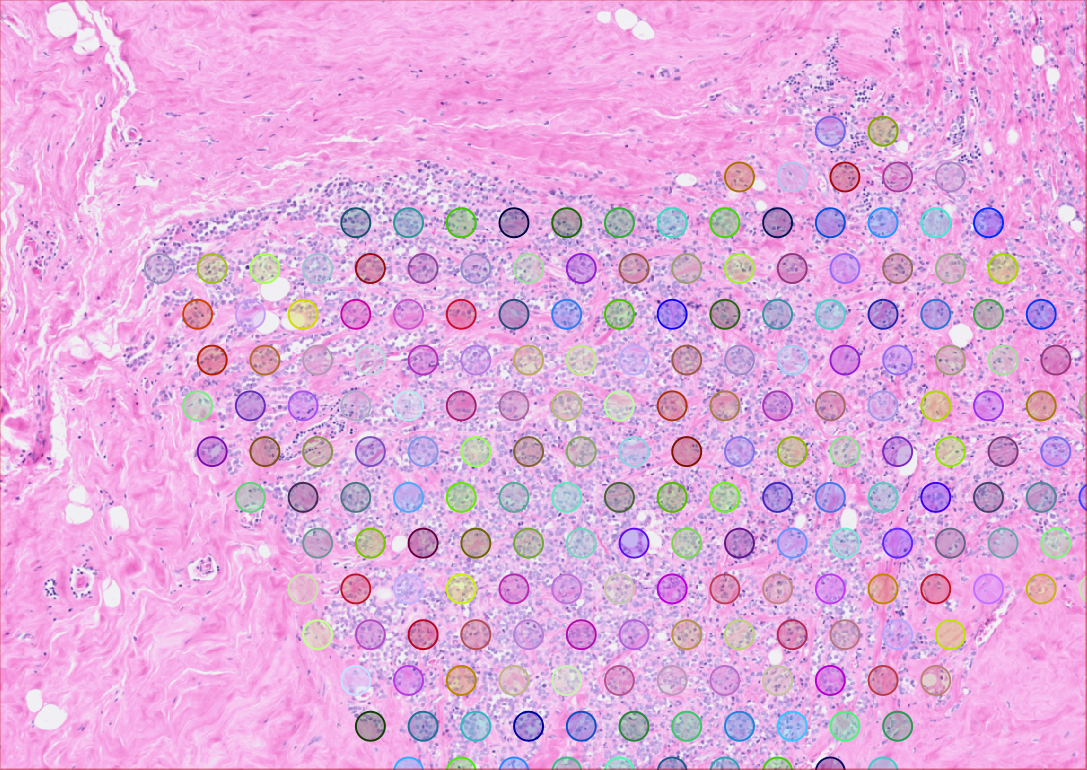
\includegraphics[width=0.45\textwidth]{result_pseudo_visium.png}
%	}\\
	\subfloat[Neighboring cell connectivity\label{fig:result_neighbor_connection}]{%
		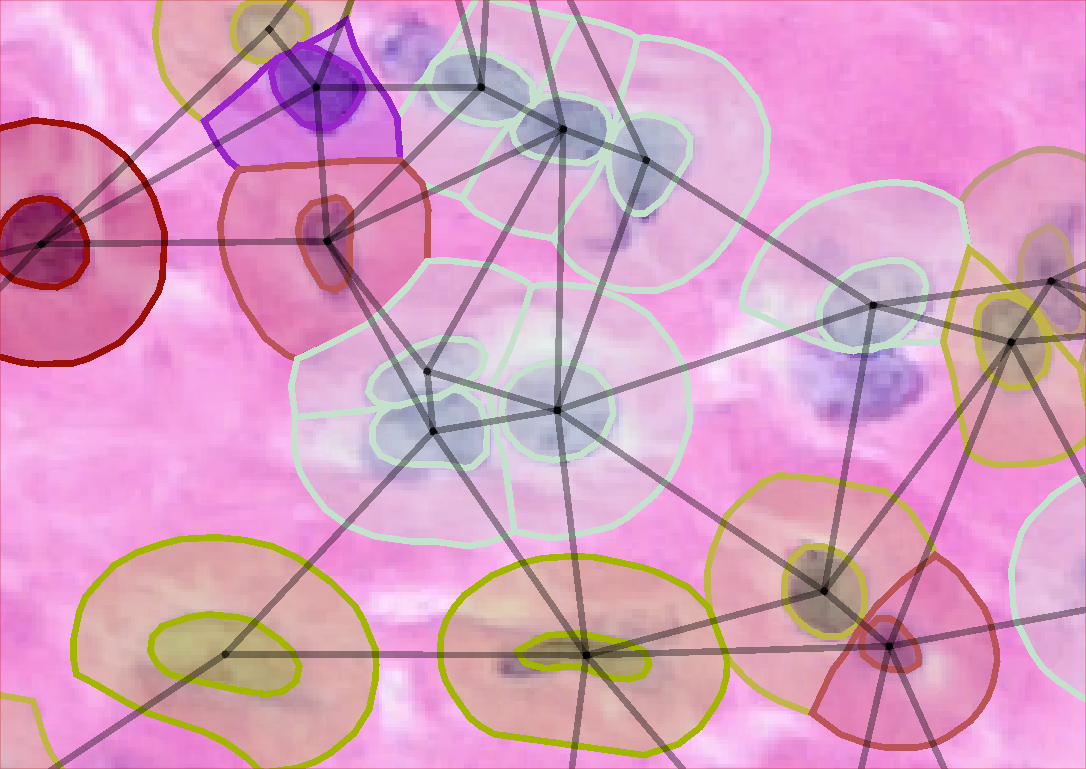
\includegraphics[width=0.45\textwidth]{result_neighbor_connection_2.png}
	}
	\hfill
	\subfloat[Distance to the boundary of a specific cell-type cluster\label{fig:result_boundary_distance}]{%
		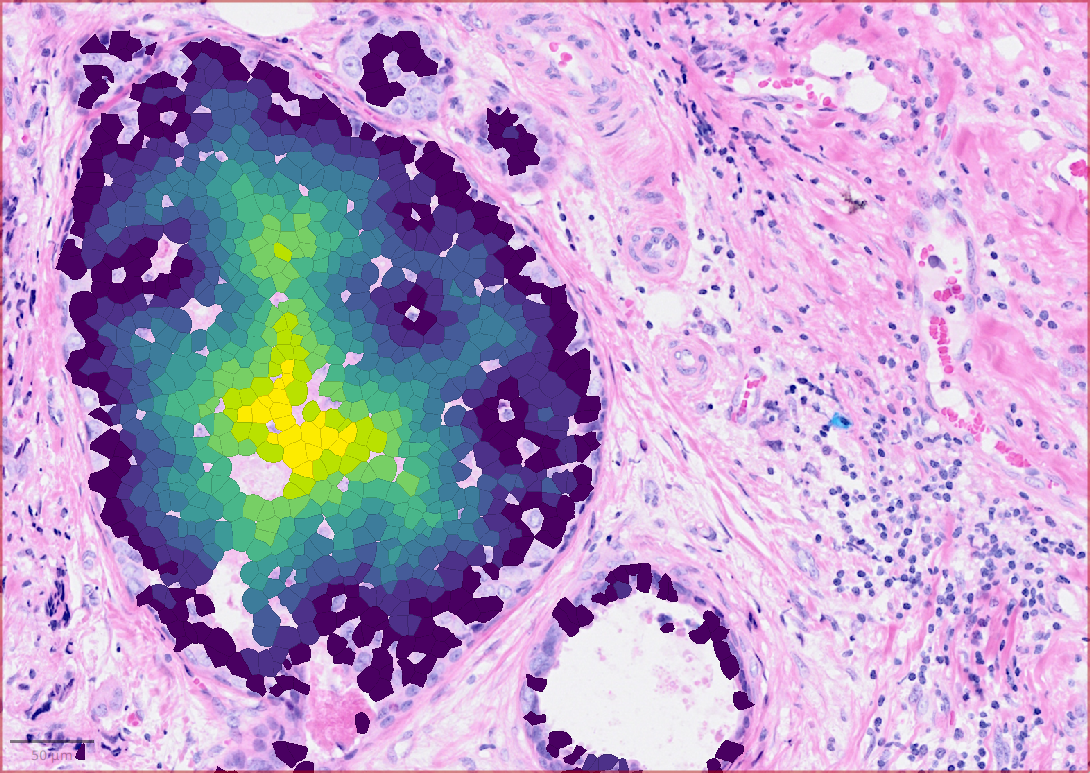
\includegraphics[width=0.45\textwidth]{result_boundary_distance.png}
	}
	\\
	\subfloat[Cell-cell interaction: MMP2->PECAM1\label{fig:result_cci_MMP2_PECAM1}]{%
		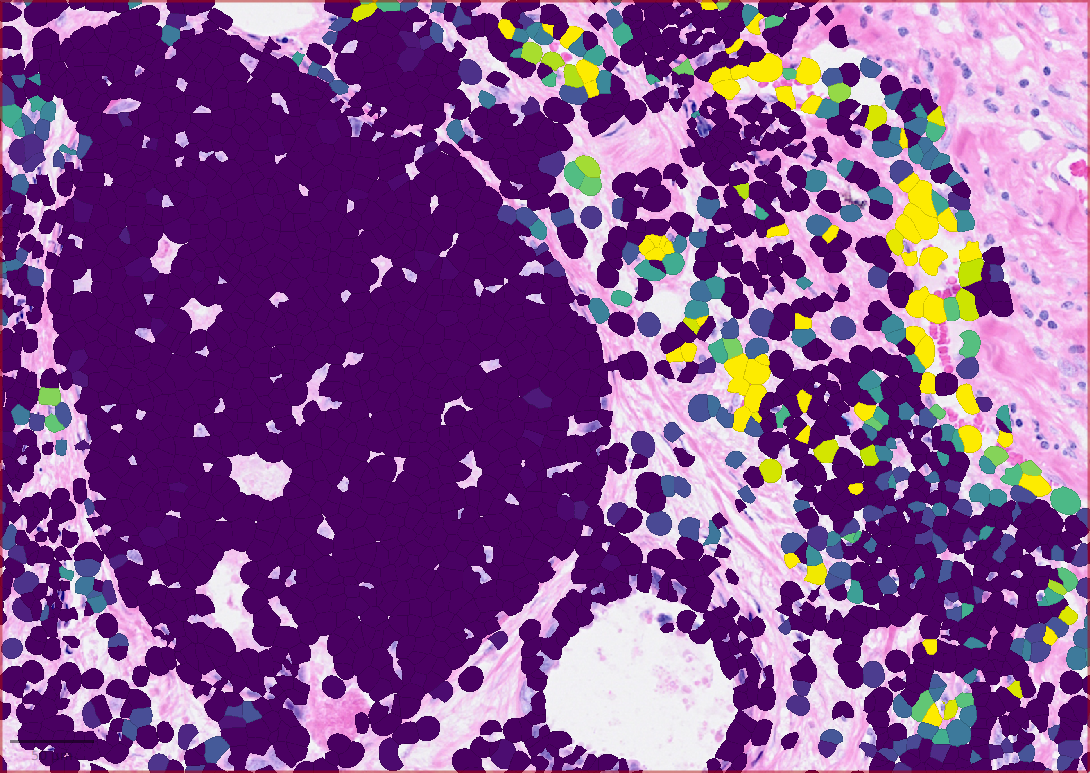
\includegraphics[width=0.45\textwidth]{result_cci_MMP2_PECAM1.png}
	}
	\hfill
	\subfloat[DBSCAN-CellX based cell clustering\label{fig:result_dbscan_cellx}]{%
		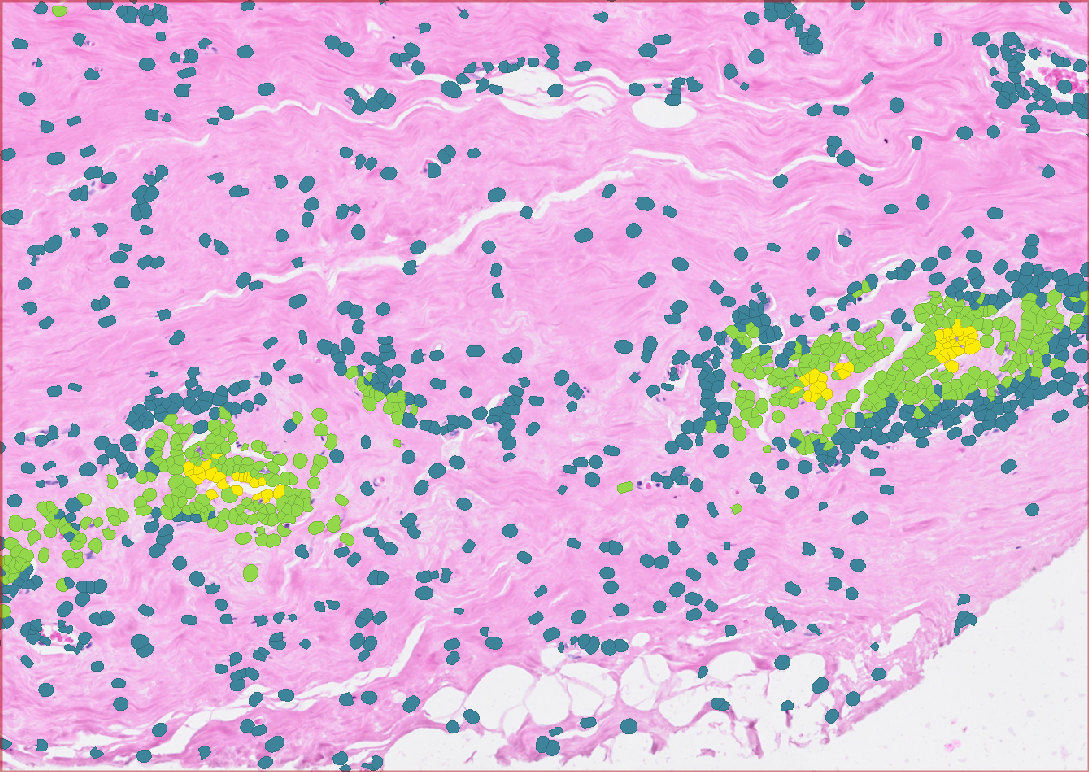
\includegraphics[width=0.45\textwidth]{result_dbscan_cellx.png}
	}
	\caption{Results showing some functions provided by QuST: (a) Neighboring cell connectivity based on Delaunay clustering. Various single cell analyses available in QuST are based on the neighboring cell connectivity.  (b) QuST's cellular spatial profiling generates a heat map indicating the distance to boundary of a specific cell type, \textit{e.g.}, tumor epithelial cells to the corresponding tumor boundary. (c) The heat map showing the cell-cell interaction intensity of the given LR pair, \textit{e.g.}, MMP2->PECAM1. (d) Result of QuST's DBSCAN-CellX implementation.}
	\label{fig:result1}
\end{figure}



\begin{figure}[htp]
	\subfloat[Raw image\label{fig:result_regseg_raw}]{%
		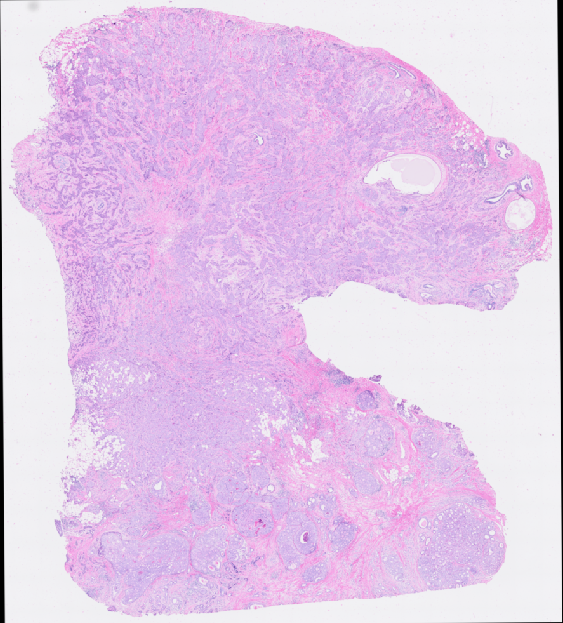
\includegraphics[width=0.3\textwidth]{result_regseg_raw.png}
	}
	\hfill
	\subfloat[Tumor regions\label{fig:result_regseg_tumor_prob}]{%
		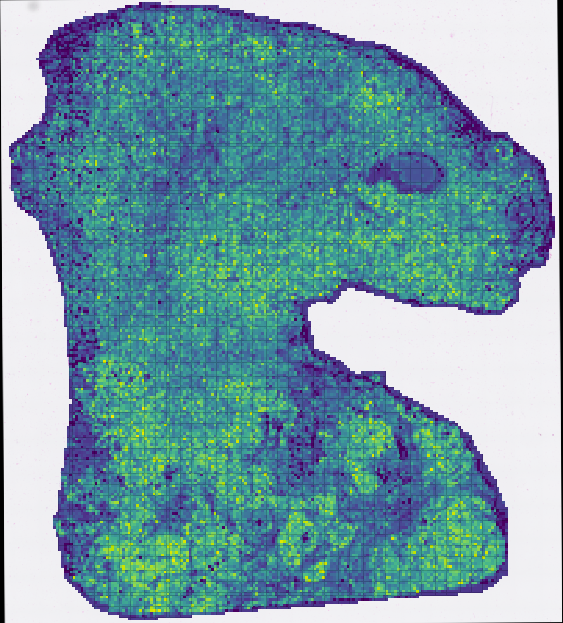
\includegraphics[width=0.3\textwidth]{result_regseg_tumor_prob.png}
	}
	\hfill
	\subfloat[Immuno regions\label{fig:result_regseg_immuno_prob}]{%
		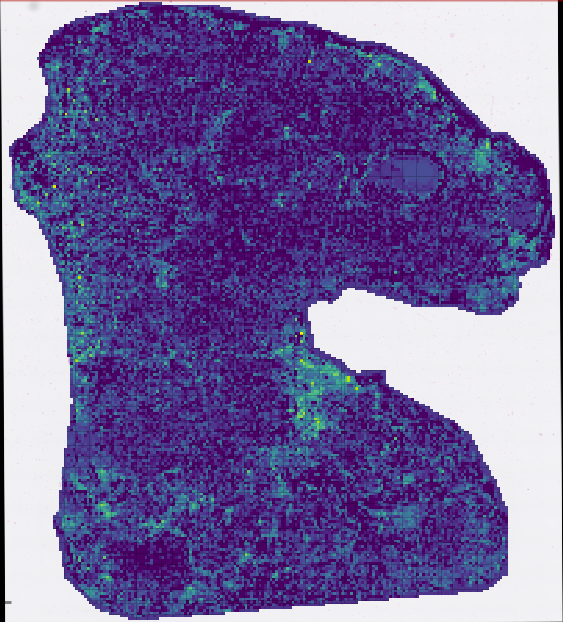
\includegraphics[width=0.3\textwidth]{result_regseg_immuno_prob.png}
	}\\
	\subfloat[Stroma regions\label{fig:result_regseg_stroma_prob}]{%
		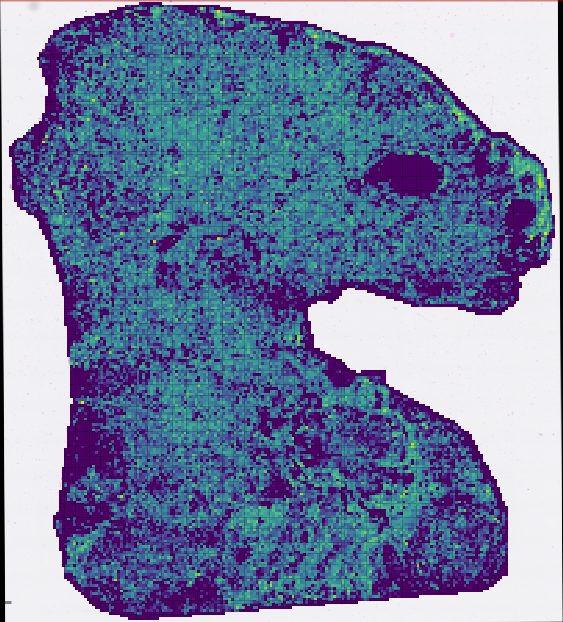
\includegraphics[width=0.3\textwidth]{result_regseg_stroma_prob.png}
	}\hfill
	\subfloat[Adipose regions\label{fig:result_regseg_adipose_prob}]{%
		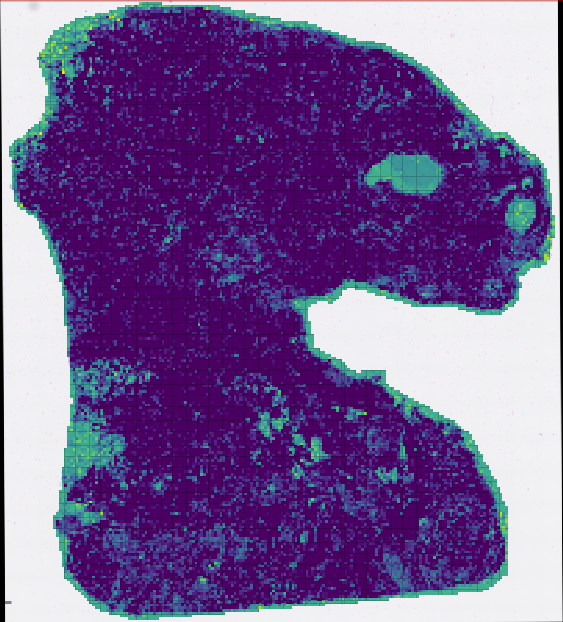
\includegraphics[width=0.3\textwidth]{result_regseg_adipose_prob.png}
	}
	\hfill
	\subfloat[Necrosis regions\label{fig:result_regseg_necrosis_prob}]{%
		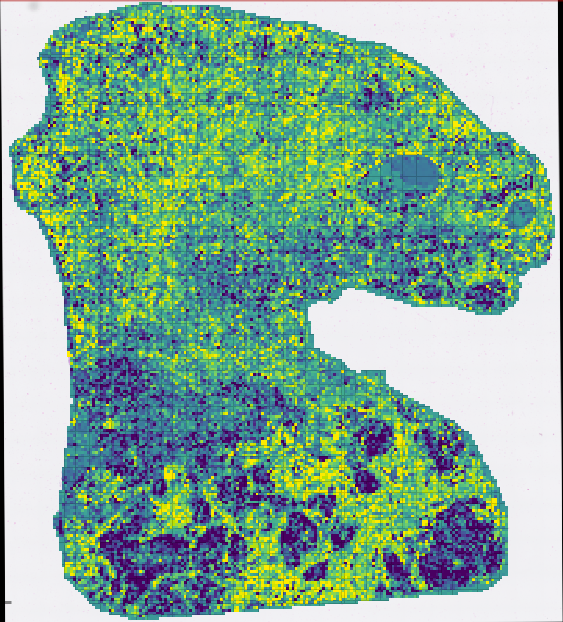
\includegraphics[width=0.3\textwidth]{result_regseg_necrosis_prob.png}
	}\\	
	\caption{Results showing the probability heat map of various classification result.}
	\label{fig:result2}
\end{figure}

A use case of QuST is spatial profiling for tumor micro-environment. The tumor microenvironment encompasses the surrounding cellular and non-cellular components that interact with cancer cells. It plays a crucial role in tumor growth, progression, and response to therapy. By understanding the complex interactions between cancer cells, immune cells, stromal cells, and the extracellular matrix, researchers can identify potential targets for therapeutic intervention. Given the rich information provided by a ST dataset, the functions that QuST can provide are of paramount importance for tumor micro-environment study.

The results showing in Figure~\ref{fig:result1} represents some comprehensive analyses of the experimental data using a range of powerful functions provided by QuST. First, given the fact that many spatial biological analyses rely on cellular spatial analysis, the Delaunay clustering method implemented in QuPath is employed to generate neighboring cell connections. For example, QuST's cellular spatial profiling, which generates a heat map that indicates the boundary distance of individual cells, \textit{e.g.,} the distance from a cancer epithelial cell to the boundary of the corresponding tumor boundary. Based on the heat map, one can explore the differential gene expression patterns between the intratumoral tumor cells and the tumor cells present in the immune-invasive region, which are located on the surface of the tumor. Next, QuST's LR-product method offers an additional layer of analysis by generating a heat map that illustrates the intensity of cell-cell interaction for a specific LR pair. This heat map provides a quantitative measure of the strength and significance of communication between specific pairs of cells. Finally, a result of QuST's DBSCAN-CellX implementation is shown, which provides a comprehensive understanding of spatial relationship of the chosen cell clusters. 

In addition, with the information contained in the ST, users can easily identify different regions within tissue samples. This capability is further enhanced by the functionality provided by QuST, which allows for classification across whole slides. As a result, the combination of QuPath and ST data provides a valuable ground truth for deep learning algorithms to perform tasks such as cell classification and region segmentation. One example is showing in Figure.~\ref{fig:result2}. %This integration holds immense potential for researchers and clinicians, as it enables a more comprehensive understanding of cellular composition and spatial relationships within tissues. By leveraging these technologies, professionals can make more accurate diagnoses, develop improved treatment strategies, and make significant advancements in fields like cancer research and drug development. Moreover, the automation and streamlining of analysis processes through QuST and DL techniques can save time and resources, while also enhancing the reproducibility and reliability of results. Ultimately, the integration of QuST and DL has the power to unlock new insights and discoveries in the field of digital pathology, revolutionizing our understanding of complex biological systems.

\begin{figure}[htp]
	\centering
	\subfloat[Pseudo Visium spots\label{fig:result_pseudo_visium}]{%
		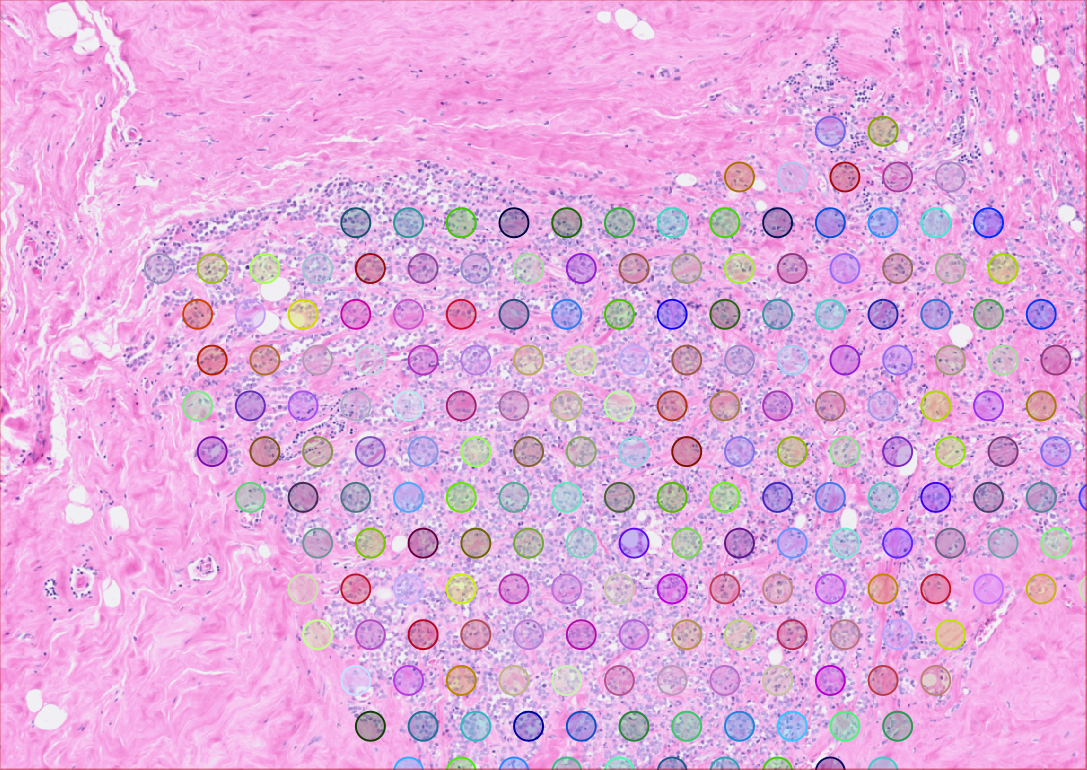
\includegraphics[width=0.45\textwidth]{result_pseudo_visium.png}
	}
	\hfill
	\subfloat[Pseudo Visium spots overlapped with single cell data \label{fig:result_pseudo_visium_sc}]{%
		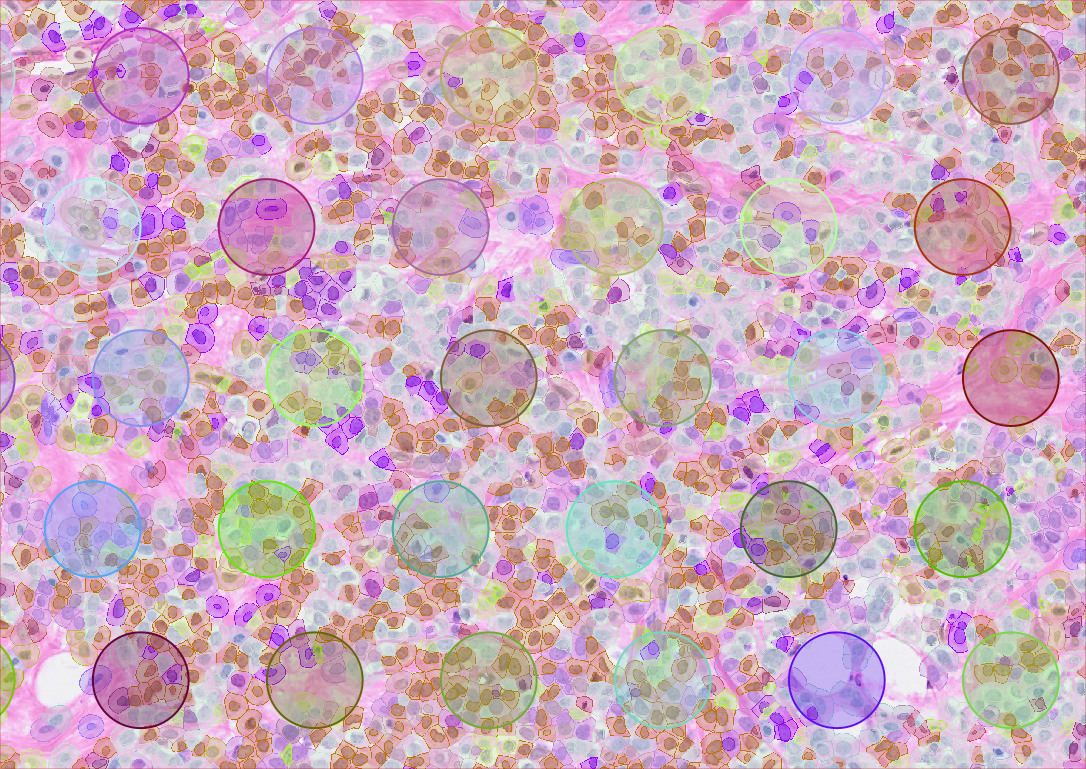
\includegraphics[width=0.45\textwidth]{result_pseudo_visium_sc.png}
	}
	\caption{Mimicking 10x Visium spots using QuST.}
	\label{fig:result3}
\end{figure}

QuST also provides an opportunity to evaluate the spatial single cell deconvolution methods by mimicking the 10x Visium datasets (see Figure~\ref{fig:result3}). For example, \cite{Huang:2023a} proposed an approach of spatial transcriptome auto-encoder and deconvolution method, largely utilizing the integration of a scalable deep generative model for predicting gene expression at cellular or nuclei level based on H\&E imaging and in situ RNA capturing, thus allowing a better understanding of the tissue microenvironment. 

Overall, the plot showcases the comprehensive analysis and visualization capabilities of QuST. QuST empowers researchers to gain a deeper understanding of the spatial relationships, boundaries, and interactions between individual cells, ultimately unraveling complex cellular dynamics and contributing to advancements in various fields of research. \footnote{The data set is freely available on 10xGenomics website: \url{https://www.10xgenomics.com/}.}

\section{Conclusion}

The QuST extension for QuPath provides a comprehensive solution for integrating whole slide image (WSI) analysis and spatial transcriptomics (ST) analysis. By leveraging the power of artificial intelligence and deep learning, QuST allows for the simultaneous analysis of molecular and morphological data, enhancing our understanding of tissue biology and pathology. The integration of ST with WSI analysis enables the visualization and exploration of gene expression patterns within the context of tissue morphology, facilitating the identification of biomarkers, therapeutic targets, and new insights into disease biology.

QuST offers a range of functionalities, including cell spatial profiling, cell-cell interaction analysis, and DBSCAN-CellX clustering. These tools enable the extraction of valuable information from ST data, such as cell neighborhood relationships and density-based clustering. Additionally, QuST incorporates DL-based image analysis for cell categorization and region segmentation, providing automated and accurate analysis of WSI data. With the QuST extension, researchers and clinicians can now seamlessly integrate WSI analysis and SY analysis within the QuPath platform. This integration enables a more comprehensive understanding of tissue biology and disease mechanisms by combining molecular information with spatial context.

In addition, QuST is able to perform cell classification and region segmentation using deep learning-based approaches. By training neural networks on annotated image patches, QuST can automatically classify cells and segment regions of interest, eliminating the need for labor-intensive manual annotation. This not only improves the efficiency of analysis but also enhances the accuracy of cell classification and region segmentation.

% The QuST extension is freely available as an open-source tool, allowing researchers and pathologists to utilize its capabilities for their spatial-omics analysis. The documentation and source code can be accessed on GitHub, along with example datasets and tutorials to support the adoption and development of QuST.

Our future works include expanding the functionality of QuST by supporting additional ST data formats, enhancing visualization tools, and integrating with other analytical platforms. By fostering community-driven resources, such as pre-trained models and example datasets, QuST aims to facilitate collaboration and the widespread adoption of ST analysis within the QuPath environment.

\section{Availability}

The QuST is developed based on QuPath 0.5.1 and Python 3.10+ and is available under the Apache 2.0 license (\url{https://github.com/huangch/qust}). A user guide is provided at \url{https://github.com/huangch/qust/user_guide}, including a step-by-step tutorials, GPU support, and examples demonstrating the use of the extension in analysis pipelines.

\bibliographystyle{unsrtnat}
\bibliography{qustwsi}  %%% Uncomment this line and comment out the ``thebibliography'' section below to use the external .bib file (using bibtex) .

\end{document}
